\chapter{Problem Formulation}\label{ch:problem_formulation}

This chapter systematically formulates the targetted task of robotic grasping as an MDP, while describing the utilised observation and action spaces alongside the applied reward function. The corresponding implementation of such formulation with detailed specifications is covered in the next \autoref{ch:implementation}.

\section{Task Definition}\label{sec:problem_formulation_task_definition}

In this work, agent is assumed to be a high-level controller that provides sequential decision making in form of gripper poses and actions. Therefore, the environment is considered to include all objects and physical interactions between in addition to the robot with its actuators and low-level controllers. Episodic formulation of the grasping task is studied, where a new set of objects is introduced into the scene at the beginning of each episode. During each episode, the aim of agent is to grasp and lift an object to a certain height above the ground plane that the objects rest on, which also terminates the current episode. Furthermore, an episode is also terminated after~100 time steps and whenever the agent pushes all objects outside the union of the perceived and reachable workspace. Placing of objects after their picking is not investigated in this work.

Due to the benefits of employing robotics simulators to train RL agents, e.g.~safe and inexpensive data collection, robotics simulator will be used in this work. Once an agent is trained in a virtual environment, the learned policy will subsequently be evaluated in a real-world setup via sim-to-real transfer. The conceptual setup of this work that should be similar in both domains is illustrated in \autoref{fig:problem_formulation_setup_sketch}.

\begin{figure}[ht]
    \centering
    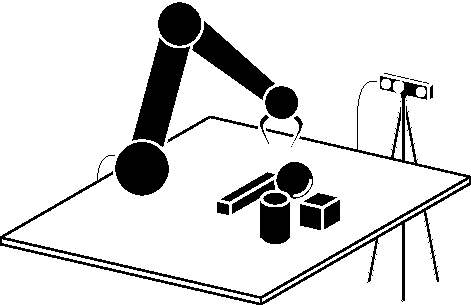
\includegraphics[width=0.65\textwidth]{problem_formulation/setup_sketch.pdf}
    \caption{Conceptual setup for the task of robotic grasping that needs to be constructed both inside a robotics simulator for training and in real-world domain for subsequent evaluation.}
    \label{fig:problem_formulation_setup_sketch}
\end{figure}


\section{Observation Space}

The observation space for the grasping task used in this work comprises of visual and proprioceptive observations. Furthermore, a set of sequential observations is stacked together for each transition in order to provide agent with temporal information about environment states.


\subsection{Octree}\label{subsec:problem_formulation_octree}

The visual observations utilised in this work are represented in form of 3D octrees. As already mentioned, the visual perception originates from a statically mounted RGB-D camera, which is assumed to provide a new RGB image and depth map of the scene at each time step. Before constructing an octree, the depth map is first used to create a point cloud of the scene as an intermediate representation. This point cloud is colourised with a corresponding RGB image that is registered to the optical frame of the camera's depth sensor. Therefore, the resulting point cloud is in form of an unstructured list of~\((x,y,z,r,g,b)\) tuples that represent individual points.

Hereafter, three assumptions about the use of volumetric 3D data representation for end-to-end robotic manipulation are set forth. First, aspect ratio of~1:1:1 is considered to provide generalisation over all possible directions of movement, i.e.~traversing a fixed distance along any of the primary axes should result in a movement over the same number of cells. Second assumption considers the volume that each cell occupies, which shall remain fixed over the entire duration of training and evaluation. This is considered to be beneficial because fixed scale of cells provides a consistency over distances between any two cells. Lastly, each cell should correspond to a specific position of space that remains fixed with respect to the robot pose, regardless of the camera pose. This assumption is considered to be necessary as it allows NNs to create relations among individual cells and their significance in space.

Due on these assumptions, the approach that is commonly used in classification and segmentation tasks, i.e.~rescale a point cloud to fit inside a fixed volume \cite{wang_o-cnn_2017}, cannot be applied in this work. However, it is assumed that the relative pose of camera with respect to robot is known, e.g.~through calibration process, therefore, the previously obtained point cloud is transformed into the robot coordinate frame in order to achieve invariance to camera pose. Furthermore, such point cloud is subsequently cropped in order to occupy a fixed volume in space with aspect ratio of~1:1:1. This volume is considered to be the observed workspace and it is subsequently used to construct the octree observations as illustrated in \autoref{fig:problem_formulation_octree_creation_sketch}.

\begin{figure}[ht]
    \centering
    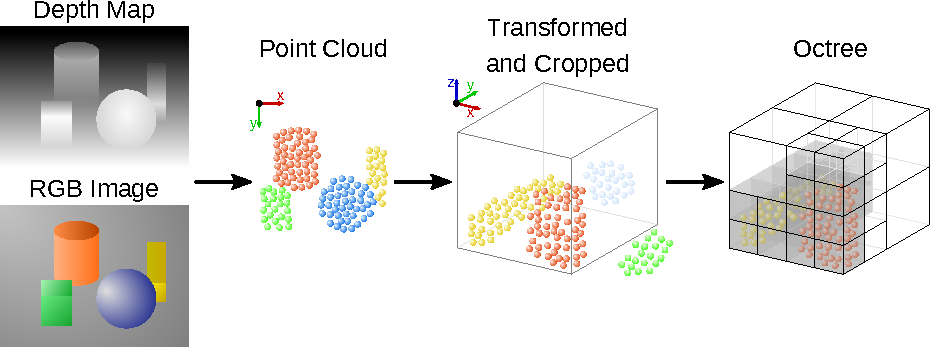
\includegraphics[width=\textwidth]{problem_formulation/octree_creation_sketch.pdf}
    \caption{Process of constructing an octree from depth map and RGB image via an intermediate point cloud, which is transformed into the robot coordinate frame and cropped to a fixed volume.}
    \label{fig:problem_formulation_octree_creation_sketch}
\end{figure}

The octree structure by \citet{wang_o-cnn_2017} allows arbitrary data to be stored at the finest leaf octants. Three distinct features are utilised in this work, namely the average unit normal vector~\(\overline{n}\), the average distance between the centre of a cell and all points that formed it~\(\overline{d}\), and the average colour~\(\overline{rgb}\). As illustrated in \autoref{fig:problem_formulation_octree_features}, all of these features are computed independently for each octant based on the points from the point cloud that produced it. Normals~\(n_{i}~{=}~(n_{x_{i}},n_{y_{i}},n_{z_{i}})\) are selected because they provide smoothness-preserving description of the object surfaces, as previously shown in \autoref{fig:rw_ocnn_occupancy_vs_normals}. Since point cloud acquired from RGB-D camera does not usually contain normals, they must be estimated from a local neighbourhood prior to constructing the corresponding octree. The average distance to the points~\(\overline{d}\) allows the perceived surface to be offset in the direction of normals, which allows octrees with lower resolution to be used while still preserving smooth transitions between the cells. Colour features~\(rgb_{i}~{=}~(r_{i},g_{i},b_{i})\) are expected to provide an agent with additional input that could allow semantic analysis in addition to shape analysis, which might be especially beneficial for distinguishing dissimilar objects that are in contact. Besides~\(\overline{n}\) being normalised as a unit vector,~\(\overline{d}\) and all channels of~\(\overline{rgb}\) are normalised to be in a range~\([0,1]\).

\begin{figure}[ht]
    \centering
    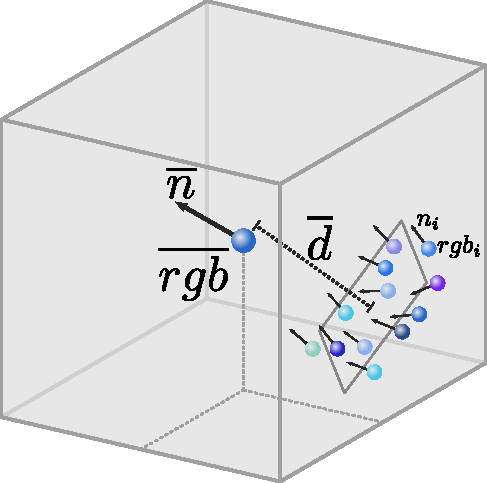
\includegraphics[width=0.4\textwidth]{problem_formulation/octree_features_sketch.pdf}
    \caption{Representation of features for a single finest leaf octant from an octree. All points from the source point cloud that belong to a cell are used to determine the average unit normal vector~\(\overline{n}\), average distance to the centre of the cell~\(\overline{d}\) and the average colour~\(\overline{rgb}\).}
    \label{fig:problem_formulation_octree_features}
\end{figure}


\subsection{Proprioceptive Observations}\label{subsec:problem_formulation_proprioceptive_observations}

In addition to the visual observations acquired by an RGB-D camera, it is considered to be beneficial to also include proprioceptive observations. Gripper pose and gripper state are used in this work because these observations are independent of the utilised robot. Although both of these could be determined solely from the visual observations, occlusion can introduce significant uncertainty. Furthermore, these readings are easily obtainable from any robot. The state of the gripper~\(g_{s}\) is represented as~\(\{closed: -1, opened: 1\}\). The position of the gripper is encoded as~\((x,y,z)\) vector represented with respect to robot's base frame. Gripper orientation is also with respect to robot's base frame, and represented as the first two columns of the rotation matrix~\([(R_{11},R_{21},R_{31}),(R_{12},R_{22},R_{32})]\) because they provide continuous description of 3D orientation without ambiguities, contrary to Euler angles or quaternions \cite{zhou_continuity_2020}.


\subsection{Observation Stacking}\label{subsec:observation_stacking}

A single set of visual and proprioceptive observations does not fully describe the state of the environment. In order to better satisfy Markov assumption, dynamics of the system must also be observed, including all data based on the temporal information. \citet{mnih_human-level_2015} addressed this in a simple way by stacking last~\(n\) historical observations together and combining them into a single observation that fully describes the state.

Despite the increase in the amount of similar data that needs to be processed, this work applies a similar observation stacking method due to the simplicity of such solution. More specifically, three sequential octrees and proprioceptive observations are stacked together, i.e.~\(n\)~=~\(3\). At the beginning of each episode when three observations are not available yet, the first observations is duplicated multiple times to form the stacked observation.


\section{Action Space}

In this work, the action space for end-to-end robotic grasping comprises of continuous actions in Cartesian space. By utilising actions in Cartesian space instead of joint space, the action space is invariant to the specific kinematic configuration of a robot. Furthermore, Cartesian actions provide better safety guarantees, where traditional IK and motion planning approaches can be employed to reliably provide commands for low-level joint controllers while avoiding self-collisions.

The utilised actions are illustrated in \autoref{fig:problem_formulation_action_space}. For gripper pose, the actions comprise of translational displacement~\((d_{x},d_{y},d_{z})\) and relative rotation around~\(z\)-axis~\(d_{\phi}\) that are both expressed with respect to robot base coordinate frame. These actions are normalised in the range~\([-1, 1]\) and subsequently rescaled to metric and angular units before applying them. The gripper action~\(g\) is also in a continuous range~\([-1, 1]\), where positive values open the gripper and negative values prompt closing of the gripper. Therefore, RL agent is allowed to take any combination of continuous actions by selecting the corresponding values for a tuple~\((d_{x},d_{y},d_{z},d_{\phi},g)\).

\begin{figure}[ht]
    \centering
    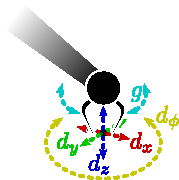
\includegraphics[width=0.333\textwidth]{problem_formulation/action_space.pdf}
    \caption{Action space of the grasping task, where~\((d_{x},d_{y},d_{z})\) indicates a translational displacement,~\(d_{\phi}\) is a relative yaw rotation, and the gripper closing and opening is denoted by~\(g\).}
    \label{fig:problem_formulation_action_space}
\end{figure}


\section{Reward Function}

Although it would be desirable to provide the agent only with a very sparse reward after successfully grasping and lifting an object, such approach would prolong the training due the sparsity of achieving a success through random exploration. Therefore, this work makes use of a composite reward function that combines together sparse rewards from four distinct stages, i.e.~reaching, touching, grasping and lifting. These stages follow a hierarchical flow, where the agent must first approach an object, then touch, grasp and finally lift it. During each episode, the agent is allowed to obtain a reward from each of these stages only once in order to discourage any rewarding behaviour that would not lead to a desired goal of the final stage, such as repeatedly pushing an object in order to continually accumulate reward for touching.

The proportion and scale of each component from the reward function can be treated as a tunable environment hyperparameter because it directly influences the policy that the agent aims to optimise. Generally, reward at the last stage should be much higher than the reward given at first stage, which is only meant to guide the training of the agent. Therefore, an exponential function~\(r_{exp}^{i-1}\) is used to determine the individual reward for each stage~\(i\). The base~\(r_{exp} \in [1,\infty)\) can be tuned, where~\(r_{exp}\)~=~\(7\) was empirically found to provide satisfactory results for the implemented grasping task, with theoretical maximum achievable reward of~\(r_{max}\)~=~\(400\).

In addition to positive reward for accomplishing the task, the agent is also given negative reward of~\(-1\) for each time step during which the robot is in collision with the ground plane in order to discourage the number of undesired collisions. Furthermore, a small reward of~\(-0.005\) is subtracted at each time step until termination in order to encourage the agent to accomplish the task as fast as possible. All rewards are summarised in \autoref{tab:reward_function}.

\begin{table}[ht]
    \centering
    \begin{tabular}{cr|lc}
        \multirow{4}{*}{\rotatebox[origin=c]{90}{\textbf{Composite}}} & \textbf{Reaching} & \(r_{exp}^{0}\)~=~\(1\)                    & \multirow{4}{*}{\textit{(once per episode)}} \\
                                                                      & \textbf{Touching} & \(r_{exp}^{1}\)~=~\(7\)                    &                                              \\
                                                                      & \textbf{Grasping} & \(r_{exp}^{2}\)~=~\(49\)                   &                                              \\
                                                                      & \textbf{Lifting}  & \(r_{exp}^{3}\)~=~\(343\)                  &                                              \\ \hline
        \multicolumn{2}{r|}{\textbf{Collision}}                       & \(-1\)            & \multirow{2}{*}{\textit{(each time step)}}                                                \\
        \multicolumn{2}{r|}{\textbf{Act Quickly}}                     & \(-0.005\)        &                                                                                           \\
    \end{tabular}
    \caption{Overview of the reward function that is utilised in this work for the grasping task, where~\(r_{exp}\)~=~\(7\) was tuned and each episode has at most~100 time steps.}
    \label{tab:reward_function}
\end{table}
